\documentclass{article}
\usepackage[main,nonanonymous]{neurips_2026}
\usepackage[utf8]{inputenc}
\usepackage[T1]{fontenc}
\usepackage{hyperref}
\usepackage{url}
\usepackage{booktabs}
\usepackage{xcolor}
\usepackage{microtype}
\usepackage{amsmath}
\usepackage{array}
\usepackage{graphicx}

\title{Midpoint Report: Parkinson's-Associated Voice Patterns, a Participant-Level Comparison of Acoustic Features and Deep Audio Representations}
\author{
  Poorav Rawat \\
  Department of Computer Science \\
  \texttt{prawat2@gsu.edu}
  \And
  Arhaan Keshwani \\
  Department of Computer Science \\
  \texttt{akeshwani2@gsu.edu}
}

\begin{document}
\maketitle

\begin{abstract}
This report summarizes progress at the midpoint of our project comparing three ways of detecting Parkinson's disease (PD)-associated patterns in sustained-vowel recordings: acoustic features with logistic regression, a compact log-Mel CNN, and a linear head on frozen wav2vec 2.0 embeddings. Controlled access to the planned mPower data was not available in time, and the feature-only UCI fallback could not support the two audio models. We therefore moved to the Italian Parkinson's Voice and Speech dataset, which provides raw audio under an open license. We have built a reproducible data pipeline that downloads and repairs the dataset, reconstructs participant identities from file names, assigns participants (not recordings) to five stratified cross-validation folds, and produces 494 cleaned, fixed-length 16\,kHz vowel clips from 47 participants. We describe the issues found along the way, most importantly duplicated participants across folders and a sample-rate difference between groups, and how each was handled. No model has been trained yet; model training and evaluation are the next stage.
\end{abstract}

\section{Project recap}
Speech can change with PD, and sustained phonation (``aaah'') is a relatively standardized task for studying it. Our research question is unchanged from the proposal: \emph{can models distinguish PD from control sustained-vowel recordings of unseen participants, and do spectrogram or frozen pretrained speech representations improve participant-level discrimination over handcrafted acoustic features under the same cohort and split?} The three planned models are (1) pitch, jitter, shimmer, harmonic-to-noise ratio, and MFCC summaries with regularized logistic regression; (2) a two-to-three-block CNN on log-Mel spectrograms; and (3) pooled wav2vec 2.0 embeddings \citep{baevski2020} with a regularized linear head. The primary metric is participant-level AUROC, with participant-bootstrap confidence intervals. The core rule is that all recordings of a person stay on the same side of every train/test split.

\section{Change of dataset}
The proposal named mPower \citep{bot2016} as the primary source and the UCI replicated-acoustic-features dataset \citep{uci489} as a fallback. Two problems led us to change this plan:
\begin{itemize}
  \item \textbf{mPower access was not granted in time.} It requires a verified Synapse profile, certification, and an approved data-use statement. Waiting would have left too little time for experiments.
  \item \textbf{The UCI fallback has no audio.} It releases precomputed features only, so it could test the acoustic model but not the CNN or wav2vec models, which are the core of our comparison.
\end{itemize}
We chose the \textbf{Italian Parkinson's Voice and Speech} dataset \citep{dimauro2019}, released under CC BY 4.0 and mirrored on Kaggle. It contains raw WAV recordings of sustained vowels (/a/, /e/, /i/, /o/, /u/, each repeated twice) and several reading tasks from clinically diagnosed PD patients and healthy controls. Unlike mPower, labels are clinical rather than self-reported, but the cohort is much smaller. The research question and the three models are unchanged.

\section{Progress so far}
\subsection{Reproducible pipeline}
All data work is done by four scripts run in order, with dependencies pinned via \texttt{uv}. Raw and derived data are git-ignored; the scripts rebuild them from scratch.
\begin{enumerate}
  \item \texttt{00\_download.py}: downloads the dataset and applies the fixes in Section~\ref{sec:issues}. We verified on a fresh copy that it reproduces exactly the files we had cleaned by hand.
  \item \texttt{01\_manifest.py}: one row per recording with participant ID, label, task, repetition, sex, birth year, sample rate, and duration. It asserts that no participant has two labels and that the expected participant counts are found.
  \item \texttt{02\_folds.py}: assigns each \emph{participant} to one of five folds, stratified by label, with a fixed seed.
  \item \texttt{03\_clean\_vowels.py}: produces the cleaned vowel clips used by all three models (Figure~\ref{fig:clips}).
\end{enumerate}

\subsection{Cohort}
The dataset has three groups: 15 young healthy controls, 22 elderly healthy controls, and a PD group. We excluded the young controls because they are much younger than the PD group, so a model could learn age instead of disease; their recordings also lack vowels and their file names do not identify the speaker. Table~\ref{tab:cohort} summarizes the remaining cohort. Healthy and PD participants have similar birth years (median 1949 vs.\ 1947), which reduces the risk of an age shortcut, but the PD group has more men.

\begin{table}[t]
\caption{Cohort after excluding young controls. Counts are participants unless stated.}
\label{tab:cohort}
\centering
\small
\begin{tabular}{lcc}
\toprule
 & Elderly healthy & PD \\
\midrule
Participants & 22 & 25 \\
Female / male & 12 / 10 & 9 / 16 \\
Birth year, median (range) & 1949 (1940--1957) & 1947 (1937--1977) \\
All recordings & 349 & 437 \\
Cleaned 3\,s vowel clips & 220 & 274 \\
Participants with 44.1\,kHz recordings & 0 & 10 \\
\bottomrule
\end{tabular}
\end{table}

\subsection{Participant-level splits}
With only 47 participants, the proposed 70/15/15 split would leave about seven people in each of the validation and test sets, giving very noisy estimates. We instead use stratified five-fold cross-validation over participants: each fold holds 9--10 people (4--5 healthy and 5 PD), and every participant is tested exactly once. Hyperparameters and thresholds will be selected by inner cross-validation within the training participants of each outer fold, so the held-out fold is never used for any choice. This matches the grouped design we had planned for the small UCI fallback.

\subsection{Vowel preprocessing}
Each vowel recording is processed independently, with no statistics shared across recordings, so preprocessing cannot leak information between folds:
\begin{enumerate}
  \item load as mono and resample to 16\,kHz (the rate wav2vec 2.0 expects);
  \item trim leading and trailing silence (30\,dB below peak);
  \item keep the middle 3\,s, the steadiest part of the vowel;
  \item scale so the peak amplitude is 0.9, since microphone distance and gain were not controlled.
\end{enumerate}
This yields 494 of 495 vowel recordings; one clip had less than 3\,s of voice after trimming and was dropped. All three models will use these same clips and the same folds, so differences in results can be attributed to the representation rather than the data.

\begin{figure}[t]
\centering
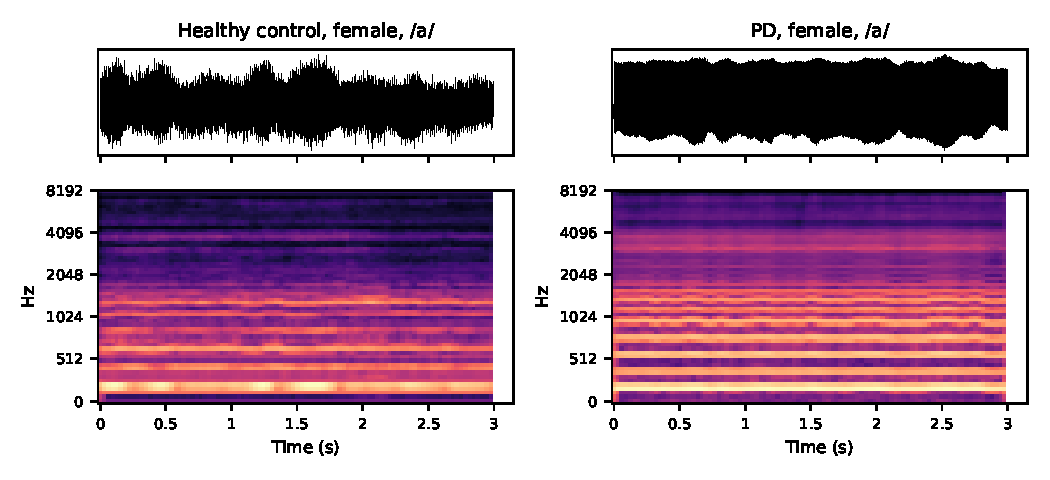
\includegraphics[width=\linewidth]{clips.pdf}
\caption{One cleaned 3\,s /a/ clip per group (both female, both originally 16\,kHz): waveform (top) and log-Mel spectrogram (bottom), the input to the CNN. Single examples are illustrative only.}
\label{fig:clips}
\end{figure}

\section{Issues and difficulties}
\label{sec:issues}
\textbf{Data access.} As described above, mPower access did not arrive in time, which forced a dataset change and a reworked split design.

\textbf{Download problems.} The Kaggle archive contains a full duplicate copy of the dataset nested inside itself, and one folder contains a copy of another participant's files. The standard macOS \texttt{unzip} also fails on a folder name with an accented character. The download script removes the duplicates and extracts with Python, renaming that folder.

\textbf{Folders are not participants.} The PD group has 28 folders but only 25 people: three patients were recorded in both 2016 and 2017 and appear in two folders. Splitting by folder would have put the same person in training and testing, inflating results. We instead build participant IDs from the code in each file name (scrambled initials, birth year, sex). This raised further problems: the initials are scrambled in a different order across sessions (we sort the letters), one file name drops an underscore in the code, two healthy men share the same initials (birth year and sex separate them), and one recording lists a birth year of 1963 for a participant whose other 15 files say 1952. Each case is handled explicitly in the manifest script, which then asserts the expected counts of 22 healthy and 25 PD participants.

\textbf{Recording-condition confound.} All 2016 PD recordings (10 participants) were made at 44.1\,kHz, while every healthy recording is 16\,kHz. A model could learn to detect the recording setup rather than the disease. Resampling everything to 16\,kHz removes the most obvious cue, but a different microphone or room may still leave traces. After training, we will repeat the evaluation on recordings that were originally 16\,kHz only; a large drop would indicate the model relies on recording conditions.

\textbf{Small cohort.} Forty-seven participants is small for deep models. Repeated vowels raise the clip count to 494, but they are not independent samples. We expect wide confidence intervals and will avoid strong claims about which model is better. This also favours our frozen-encoder and small-CNN designs over training large models from scratch.

\section{Next steps}
\begin{table}[t]
\caption{Remaining work.}
\label{tab:plan}
\centering
\small
\begin{tabular}{p{0.3\linewidth}p{0.6\linewidth}}
\toprule
Step & Work \\
\midrule
Acoustic baseline & Extract pitch, jitter, shimmer, HNR, and MFCC summaries per clip; train regularized logistic regression with inner-CV tuning. \\
Log-Mel CNN & Compute log-Mel spectrograms; train a compact CNN with early stopping on inner-fold participant AUROC; train-only gain and noise augmentation. \\
Frozen wav2vec 2.0 & Extract pooled embeddings from a published checkpoint; train a regularized linear head. \\
Evaluation & Average clip scores per participant; report AUROC, balanced accuracy, sensitivity, and specificity with participant-bootstrap 95\% CIs and paired model comparisons. \\
Robustness checks & Repeat evaluation on originally-16\,kHz recordings only; report results by sex where counts allow. \\
Demo and final report & Educational demo showing waveform, spectrogram, and an experimental score with a clear non-diagnostic statement. \\
\bottomrule
\end{tabular}
\end{table}
Building and training the three models is the immediate next step (Table~\ref{tab:plan}). We will start with the acoustic baseline, since it is fastest and gives a reference point for the two deep models. The project docs, which still describe the mPower plan, will also be updated to match the new dataset and split design.

\section{Limitations}
The new dataset is small, comes from a single clinical site, and has a known recording-condition difference between groups, so results may not generalize to other populations or devices. Sustained vowels capture only one aspect of speech. As in the proposal, any model will be framed as a research tool and not as a diagnostic test.

\begin{thebibliography}{9}
\bibitem[Baevski et~al.(2020)]{baevski2020}
Baevski, A., Zhou, Y., Mohamed, A., and Auli, M. (2020).
Wav2vec 2.0: A framework for self-supervised learning of speech representations.
\emph{Advances in Neural Information Processing Systems}, 33.

\bibitem[Bot et~al.(2016)]{bot2016}
Bot, B.~M. et~al. (2016).
The mPower study, Parkinson disease mobile data collected using ResearchKit.
\emph{Scientific Data}, 3, 160011.
\url{https://doi.org/10.1038/sdata.2016.11}.

\bibitem[Dimauro and Girardi(2019)]{dimauro2019}
Dimauro, G. and Girardi, F. (2019).
Italian Parkinson's Voice and Speech.
IEEE Dataport. \url{https://doi.org/10.21227/aw6b-tg17}.

\bibitem[UCI(2019)]{uci489}
UCI Machine Learning Repository (2019).
Parkinson dataset with replicated acoustic features.
\url{https://archive.ics.uci.edu/dataset/489/parkinson+dataset+with+replicated+acoustic+features}.
\end{thebibliography}

\end{document}
